\documentclass[unicode, notheorems]{beamer}
\usepackage{etex}  % Should be second line. Otherwise tikz raises error.
\hypersetup{pdfpagemode=FullScreen}

% If you have more than three sections or more than three subsections in at least one section,
% you might want to use the [compress] switch. In this case, only the current (sub-) section
% is displayed in the header and not the full overview.
\mode<presentation>
{
  \usetheme{Madrid}
  \usecolortheme{seahorse}
}

% https://tex.stackexchange.com/questions/106789/why-does-usepackaget2afontenc-take-over
\usepackage[T2A,T1]{fontenc}
\usepackage[english]{babel}
\usepackage{amsthm}
\usepackage[noend]{algorithmic}
\usepackage{algorithm}
\usepackage[all]{xy} % for graph plotting
% \usepackage{times}
\usepackage{tikz}
\usetikzlibrary{arrows,shapes,backgrounds}
\usepackage{textcomp} % euro sign
\usepackage[official]{eurosym}
\usepackage{ulem} % strike
\usepackage{color} % use colors (in minted)

% tables
\usepackage{booktabs}
\usepackage{multirow}

%% Code highlight
% Doc: http://ftp.yzu.edu.tw/CTAN/macros/latex/contrib/listings/listings.pdf
\usepackage{listings}
\usepackage{minted}
% ftp://ftp.dante.de/tex-archive/macros/latex/contrib/minted/minted.pdf
% Note: to use minted, install pygments http://pygments.org/ and add "-shell-escape" flag to latex command.
% Minted doc: http://ftp.yzu.edu.tw/CTAN/macros/latex/contrib/minted/minted.pdf
%% END: Code highlight

% Font settings 
%\usepackage[scaled]{futura}
\usepackage{helvet}

%\usefonttheme{serif}     % Font theme: serif
%\usepackage{ccfonts}     % Font family: Concrete Math

% \usefonttheme[onlymath]{serif}
% \defaultfontfeatures{Mapping=tex-text} 
%\setsansfont[Ligatures={Common}]{Futura}
% \setmonofont[Scale=0.8]{Monaco} 

\title{Data Science with Apache Spark}
\author{Kirill Pavlov}
\institute[]{Data Science Team, Asia Miles Limited}
\titlegraphic{\includegraphics[width=4cm]{./images/logo}}
\date{\today}

\definecolor{aml_gray_light}{RGB}{147,153,157}
\definecolor{aml_gray_dark}{RGB}{39,47,56}
\definecolor{aml_yellow}{RGB}{250,207,0}

\setbeamertemplate{title page}[default][colsep=-4bp,rounded=true]
\setbeamertemplate{itemize items}[default]
\setbeamertemplate{enumerate items}[default]

\setbeamercolor*{palette primary}{use=structure,fg=white,bg=aml_gray_light}
\setbeamercolor*{palette secondary}{use=structure,fg=white,bg=aml_gray_dark}
\setbeamercolor*{palette tertiary}{use=structure,fg=white,bg=aml_yellow}

\setbeamercolor{itemize item}{fg=aml_yellow}
\setbeamercolor{itemize subitem}{fg=aml_yellow}
\setbeamercolor{enumerate item}{fg=aml_gray_dark}
\setbeamercolor{enumerate subitem}{fg=aml_gray_dark}

\setbeamertemplate{section in toc}{%
  {\color{aml_gray_dark}\inserttocsectionnumber.}~\inserttocsection}
\setbeamercolor{subsection in toc}{bg=white,fg=structure}
\setbeamertemplate{subsection in toc}{%
  \hspace{1.2em}{\color{aml_gray_dark}\rule[0.3ex]{3pt}{3pt}}~\inserttocsubsection\par}
  
% Set beamer blocks
\setbeamertemplate{blocks}[rounded][shadow=false]
\addtobeamertemplate{block begin}{\pgfsetfillopacity{0.8}}{\pgfsetfillopacity{1}}

% \setbeamercolor*{block title example}{fg=aml_gray_dark,bg= aml_gray_light}
%\setbeamercolor*{block body example}{fg= blue,bg= blue!5}
\setbeamercolor*{block title example}{fg=white,bg= aml_gray_light}
\setbeamercolor*{block body example}{fg=white,bg= aml_gray_dark}

% remove page navigation.
\beamertemplatenavigationsymbolsempty

% Set link colours
\definecolor{links}{HTML}{2A1B81}
\hypersetup{colorlinks,linkcolor=,urlcolor=links}

\begin{document}
% For every picture that defines or uses external nodes, you'll have to
% apply the 'remember picture' style. To avoid some typing, we'll apply
% the style to all pictures.
\tikzstyle{every picture}+=[remember picture]

% By default all math in TikZ nodes are set in inline mode. Change this to
% displaystyle so that we don't get small fractions.
\everymath{\displaystyle}

% This presentation shows ability of spark to work with data.
% It covers data processing, pipelining, feature engineering and algorithms available in Spark.

\begin{frame}
\titlepage
\end{frame}

\begin{frame}{Quick Questionnaire}
\begin{itemize}
\item How many people have attended previous Spark talks? \pause
\item How many people are currently working with Spark? \pause
\item How many people are familiar with Scala?
\end{itemize}
\end{frame}

\begin{frame}{About the Presenter}

\begin{columns}
\column{.7\textwidth}
  {\footnotesize 
    \begin{itemize}
    \item MS degree from Moscow Institute of Physics and Technology with distinction.
    \item 8+ years of data science and machine learning experience.
    \item Worked in Yandex (Russian Google) on search and on-line contextual ads ranking algorithms.
    \item Developed and consulted start-ups in digital marketing, healthcare, real estate and home automation areas.
    \item Open-source contributor, full-stack engineer and data mining evangelist.
    \item Now data scientist in Asia Miles.
    \end{itemize}
  }
\column{.3\textwidth}
	\includegraphics[scale=0.8]{images/author}
\end{columns}
\end{frame}

\begin{frame}{Table of content}
  % \tableofcontents[currentsection]
  \tableofcontents
\end{frame}

\section{Overview}
\frame{\tableofcontents[currentsection]}

\begin{frame}
%% Some of you may know about this picture. I would like to focus on its bottom part. My boss thinks I am working with excel. Thank is not necesserely wrong. Problem with "what I do" picture is that people do not understand it. After part with formulas we simple charts.
%% Another picture I would like to focus here is "what I actually do", particulary SQL part, which is seems to be nesessary for big data projects.
\begin{center}
\includegraphics[width=12cm]{./images/Data-Scientist-What-I-really-do}
\end{center}

{\footnotesize
source: \href{http://www.sintetia.com/wp-content/uploads/2014/05/Data-Scientist-What-I-really-do.png}{www.sintetia.com}
}
\end{frame}

\begin{frame}{Overview}
\begin{itemize}
% Data aprocessing and cleaning takes about 80% of developer's time.
% How to process big data? Use database solutions.
\item Data processing and cleaning takes \textbf{80\%} of time.
\end{itemize}
\end{frame}

\begin{frame}{Environment}
\begin{columns}
\column{.33\textwidth}
\begin{center}
	\includegraphics[scale=0.5]{images/spark-logo}
\end{center}
\column{.33\textwidth}
\begin{center}
	\includegraphics[scale=0.5]{images/scala}
\end{center}
\column{.34\textwidth}
\begin{center}
	\includegraphics[scale=0.5]{images/zeppelin}
\end{center}
\end{columns}

% * How do we work with spark in the private cloud: zeppelin. Why zeppelin?
% * We use scala. Why not python? native integration.
% * Why zeppelin? (notebook at all/compare to Jupyter)
\end{frame}

\begin{frame}{visualization}
* Data visualization part (we use excel/external 3rd party tools). Sometimes d3js.
* Data visualization split data generation from data plot. Automate genration part.
\end{frame}

\section{Data transformation and analysis with Spark}

\begin{frame}[fragile]{Example: Estimators and Transformers}

{\footnotesize
\begin{minted}[linenos,
               numbersep=2pt,
               frame=lines,
               framesep=2mm]{scala}
// Define indexers and encoders
val fieldsToIndex = Array("gender", "curr_tier_type",  "prefred_lang")
val indexers = fieldsToIndex.map(f => new StringIndexer()
  .setInputCol(f).setOutputCol(f + "_index"))

val fieldsToEncode = Array("gender", "prefred_lang")
val oneHotEncoders = fieldsToEncode.map(f => new OneHotEncoder()
  .setInputCol(f + "_index").setOutputCol(f + "_flags")) 

// Combine stages into pipeline
val pipeline = new Pipeline().setStages(indexers ++ oneHotEncoders) 
\end{minted}
}
\end{frame}

\section{Data mining with Spark}

\begin{frame}{Workflow}
\begin{center}
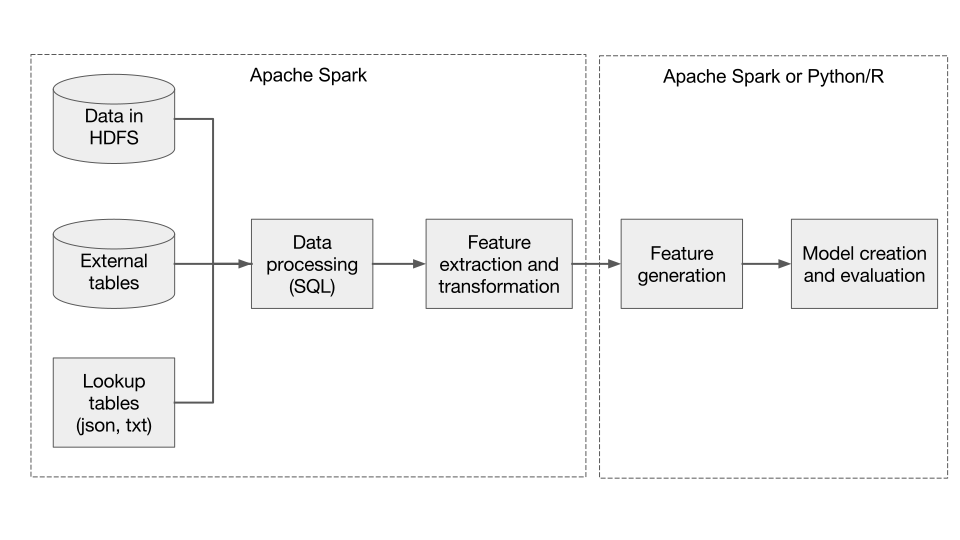
\includegraphics[width=12cm]{images/ml-workflow}
\end{center}
\end{frame}


\section{Conclusion}
\begin{frame}{Recap}
\end{frame}

\begin{frame}{Quiz}
\end{frame}

\begin{frame}{We are hiring data scientists}
\end{frame}

\begin{frame}
\begin{center}
{\huge Thank you!}

\vfill

Kirill Pavlov, Data Science Team, Asia Miles Limited

kirill\_pavlov@asiamiles.com
\end{center}
\end{frame}

\end{document}
